\documentclass[10pt,a4paper]{article}
\usepackage[utf8]{inputenc}
\usepackage{amsmath}
\usepackage{amsfonts}
\usepackage{amssymb}
\usepackage{graphicx}

\begin{document}
\title{Projet 4: pre-labo 1}
\date\today
\author{Groupe 7}
\maketitle

\section{Calcul de la différence de temps}
	Afin d'observer les répliques, une configuration a été pensée (Figure \ref{conf1} et \ref{conf2}). $d$ est la distance $Tx$ et $Rx$ alors que $x$ est la distance minimale entre $Rx$ (ou $Tx$) et la plaque. Le temps que met l'onde pour passer de $Rx$ à $Tx$ est donné par l'équation \ref{t1}. L'équation \ref{t2} donne le temps du trajet de l'onde réfléchie sur la plaque. $c$ est la vitesse de la lumière. 	

	\begin{equation}
	t_1 = \frac{d}{c}
	\label{t1}
	\end{equation}
	
	\begin{equation}
	t_2 = \sqrt{(\frac{d}{2})^2 + x^2} * \frac{2}{c}
	\label{t2}
	\end{equation}
	
	Le première situation sera réalisée pour obtenir un grand $\Delta t$ alors que la seconde pour en obtenir un plus petit.
	\begin{equation}
	\Delta t = t_2 - t_1 = (2\sqrt{(\frac{d}{2})^2 + x^2} - d ) * \frac{1}{c}
	\end{equation}
	
	\begin{figure}[h]
	\centering
	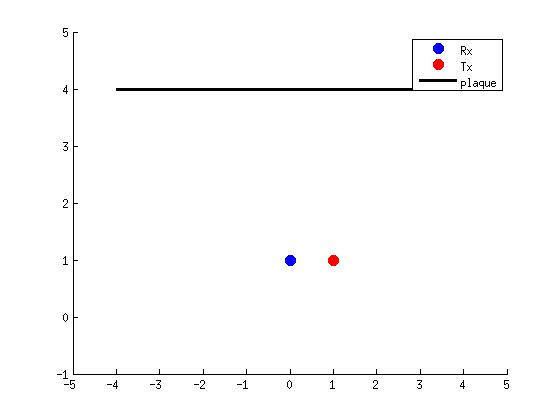
\includegraphics[scale=0.4]{conf1.jpg}
	\caption{Première configuration \label{conf1} }
	\end{figure}		
	
	\begin{figure}[h]
	\centering
	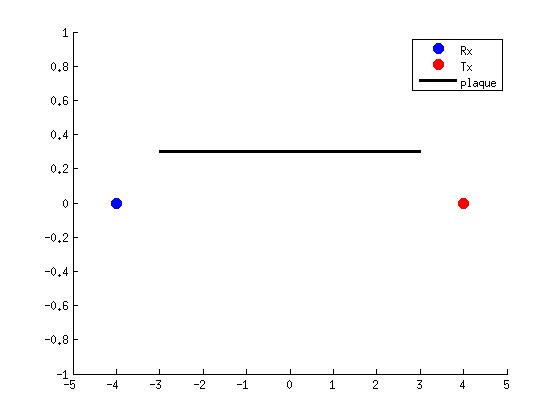
\includegraphics[scale=0.4]{conf2.jpg}
	\caption{Deuxième configuration \label{conf2}}
	\end{figure}		
	
	
	\section{Détermination des paramètres géométriques}
		Afin de ne pas avoir de recouvrement entre deux répliques d'une impulsion, il faut que $\Delta t$ soit plus grand que le temps d'une impulsion ($1ns$). De plus lors du labo il y aura des contraintes d'espace. Pour calculer les set-up les $\Delta t$ et les $d$ sont fixés. Le paramètre $x$ se trouve alors grâce aux deux précédents (Equation \ref{eq}). Les différents set-up qui seront testés se trouvent à la Figure \ref{set}.
		
		\begin{equation}
			x = \sqrt{(\frac{\Delta t c}{2})^2 + \frac{d c \Delta t}{2}}
			\label{eq}
		\end{equation}
		
		
		\begin{figure}[h]
		\centering
		\begin{tabular}{|l|l|l|l|l|l|l|}
		\hline
		 configuration & $\Delta t [ns]$ & $d [m]$ & $x[m]$ & $Rx$ & $Tx$ & $Plaque$\\
		 \hline
		 0 & $1.5$ & $2$ & $0.7073$ & $(0,0)$ & $(2,0)$ & $(1,0.7073)$ \\ 
		 1 & $3$ & $2$ & $1.0496$ & $(0,0)$ & $(2,0)$ & $(1,1.0496)$  \\
		 2 & $4$ & $2$ & $1.2485$ & $(0,0)$ & $(2,0)$ & $(1,1.2485)$ \\
		 3 & $6$ & $1$ & $1.3070$ & $(0,0)$ & $(1,0)$ & $(0.5, 1.3070)$\\
		 4 & $8$ & $0.5$ & $1.4274$ & $(0,0)$ & $(0.5,0)$ & $(0.25, 1.4274)$ \\
		 5 & $10$ & $0.5$ & $1.7310$ & $(0,0)$ & $(0.5,0)$ & $(0.25,1.7310)$ \\
		 \hline
		\end{tabular}
		
		\caption{Set-up pour le premier labo}
		\label{set}
		\end{figure}

 \section{Échantillonnage} 
 Afin de respecter le théorème de Shannon-Nyquist, nous allons échantillonner à 20GHz. On enregistre un sample toutes les 50ps. De plus nous comptons enregistrer de 100 périodes (de 106.6ns) afin de pouvoir mieux traiter le phénomène à observer. Cela nous fait donc 213200 échantillons.
\end{document}